
%(BEGIN_QUESTION)
% Copyright 2010, Tony R. Kuphaldt, released under the Creative Commons Attribution License (v 1.0)
% This means you may do almost anything with this work of mine, so long as you give me proper credit

Calculate the necessary size ($C_v$, and also pipe size in inches) control valve to pass a maximum of 2.1 SCFM of chlorine gas (specific gravity = 2.47) in this wastewater disinfection system, where enough chlorine (Cl$_{2}$) is continuously mixed with the wastewater to kill most harmful micro-organisms:

$$\includegraphics[width=15.5cm]{i04362x01.eps}$$

A pressure regulator connected to the chlorine source regulates the control valve's upstream pressure at a constant $-30$ inches water column, while a venturi-shaped {\it eductor} uses the flow of wastewater to create a vacuum to pull chlorine gas into the water with a pressure of $-120$ inches water column.  Assume a temperature of 50$^{o}$ F, a single-port ported-plug control valve, and negligible friction in the chlorine gas piping.

\vskip 10pt

$C_v$ = \underbar{\hskip 50pt} \hskip 100pt Nominal pipe size = \underbar{\hskip 50pt} inches

\vskip 10pt

\underbar{file i04362}
%(END_QUESTION)





%(BEGIN_ANSWER)

$C_v$ = \underbar{\bf 0.5257} \hskip 50pt Nominal pipe size = \underbar{\bf 1/4} inch (0.235 inches calculated)

\vskip 10pt

%(END_ANSWER)





%(BEGIN_NOTES)

Since chlorine in this example is a gas, not a liquid, we will use the following gas valve sizing formula:

$$Q = 963 \> C_v \sqrt{{\Delta P (P_1 + P_2)} \over {G_g T}}$$

\noindent
Where,

$Q$ = Gas flow rate, in units of Standard Cubic Feet per Hour (SCFH)

$C_v$ = Valve capacity coefficient

$\Delta P$ = Pressure dropped across valve, pounds per square inch differential (PSID)

$P_1$ = Upstream valve pressure, pounds per square inch absolute (PSIA)

$P_2$ = Downstream valve pressure, pounds per square inch absolute (PSIA)

$G_g$ = Specific gravity of gas (Air at standard temperature and pressure = 1.0)

$T$ = Absolute temperature of gas in degrees Rankine ($^{o}$R)

\vskip 10pt

First, manipulating the formula to solve for $C_v$:

$$C_v = {Q \over 963 \sqrt{{\Delta P (P_1 + P_2)} \over {G_g T}}}$$

Next, we need to express the pressures and temperatures in their proper units:

\vskip 10pt

$P_1$ = -30 "WC = -1.084 PSIG = {\bf 13.62 PSIA}

\vskip 10pt

$P_2$ = -120 "WC = -4.335 PSIG = {\bf 10.36 PSIA}

\vskip 10pt

$T$ = 50 $^{o}$F = 509.67 $^{o}$R 

\vskip 10pt

$Q$ = 2.1 SCFM = 126 SCFH 

\vskip 10pt

Lastly, we plug in these values and solve for $C_v$:

$$C_v = {126 \over 963 \sqrt{{(13.62 - 10.36) (13.62 + 10.36)} \over {(2.47) (509.67)}}} = 0.5257$$

Now that we know the value of $C_v$, we can solve for the nominal pipe size by taking the $C_d$ value for a single-port, port-guided globe valve (9.5) and using the appropriate formula:

$$C_d = {C_v \over d^2}$$

$$d^2 = {C_v \over C_d}$$

$$d = \sqrt{C_v \over C_d}$$

$$d = \sqrt{0.5257 \over 9.5} = 0.235 \hbox{ inches}$$

Thus, a 1/4 inch nominal pipe size valve should work for this application.

%INDEX% Final Control Elements, valve: sizing

%(END_NOTES)


